\documentclass[12pt]{mwart}

\usepackage{polski}
\usepackage[utf8]{inputenc}
\usepackage{graphicx,float,enumitem, bm}
\usepackage{tabularray}
\mathtoolsset{mathic}
\raggedbottom
\graphicspath{ {./images/} }

\author{Mateusz Stasiak \\ Indeks: 262339}
\title{Weryfikacja hipotez statystycznych}

\begin{document}
	\maketitle
	
	\section{Zadanie 1}
	\subsection{Wstęp}
	\noindent Hipotezą zerową nazywamy założenie, że wartość średnia $\mu$ naszych danych wyniesie $1.5$. Hipotezę tę oznaczamy symbolem $H_0$ i piszemy $H_0 \colon \mu = \mu_0 = 1.5$. Drugą hipotezę nazywamy hipotezą alternatywną i oznaczamy ją przez $H_1$. W naszym przypadku:
	\begin{enumerate}[label=(\alph*)]
		\item $H_1 \colon \mu \neq \mu_0$
		\item $H_1 \colon \mu > \mu_0$
		\item $H_1 \colon \mu < \mu_0$. \\
	\end{enumerate} 
	
	\noindent Jeśli zachodzi hipoteza zerowa, to nasze dane mają rozkład $N(1.5,0.2)$. Do weryfikacji $H_0$ będziemy potrzebować jakiejś statystyki testowej. Zauważmy, że parametr $\sigma$ jest znany i wynosi $0.2$, dlatego mądrym pomysłem będzie wykorzystanie średniej z dostępnych obserwacji. Ta zmienna losowa $\overline{X}$ ma rozkład $N(\mu,\frac{\sigma}{\sqrt{n}})$. Zatem najwygodniej będzie dodatkowo przeprowadzić standaryzację tej średniej i użyć statystyki $$Z = \cfrac{\overline{X}-\mu_{0}}{\sigma_{\overline{X}}} = \cfrac{\overline{X}-\mu_{0}}{\frac{\sigma}{\sqrt{n}}}, \qquad Z \sim N(0,1).$$
	
	
	\noindent Gdy hipoteza zerowa $H_0$ jest fałszywa, wzór na statystykę $Z$ można zapisać następująco:
	$$ Z = \cfrac{\overline{X}-\mu_{0}}{\frac{\sigma}{\sqrt{n}}} = \underbrace{\cfrac{\overline{X}-\mu_{0}}{\frac{\sigma}{\sqrt{n}}}}_{\sim N(0,1)} + \cfrac{\mu-\mu_{0}}{\frac{\sigma}{\sqrt{n}}}.$$ 
	
	
	\noindent Ze wzoru widać, że kluczem do weryfikacji hipotezy jest sprawdzenie czy statystyka $Z$ przyjmuje wartości charakterystyczne dla założonego rozkładu $N(0,1)$. Jeśli nie, to niepoprawny będzie również rozkład przewidywany dla $\overline{X}$, a tym samym odrzucimy naszą hipotezę zerową. Zbiór liczb, które prowadzą do odrzucenia hipotezy $H_0$ na korzyść $H_1$ nazywamy zbiorem krytycznym $C$. Jego rozmiar zależy od miary dokładności wykonywanego testu, czyli tzw. poziomu istotności. Wyznacza on prawdopodobieństwo popełnienia błędu pierwszego rodzaju - odrzucenia hipotezy zerowej, gdy jest ona prawdziwa. Poziom istotności oznaczamy poprzez symbol $\alpha$. W zadaniu przyjmujemy, że jest on równy $0.05$.
	
	
	\noindent Wprowadźmy jeszcze pojęcie p-wartości. Jest to najmniejszy poziom istotności $\alpha$, przy którym zaobserwowana wartość statystyki testowej $Z$ prowadzi do odrzucenia hipotezy zerowej $H_0$.

	
	\subsection{Hipoteza alternatywna $\bm{H_1 \colon \mu \neq 1.5}$, $\bm{\alpha=0.05}$}
	\noindent Z teorii estymacji przedziałowej dla danych z rozkładu normalnego wiemy, że $P_{H_0}(z_{\frac{\alpha}{2}} \leq Z \leq z_{1-\frac{\alpha}{2}})= P_{H_0}(-z_{1-\frac{\alpha}{2}} \leq Z \leq z_{1-\frac{\alpha}{2}}) = 1 - \alpha$. Powyższe kwantyle rozkładu $N(0,1)$ wynoszą $z_{0.025}=-1.96$ oraz $z_{0.975}=1.96$. Zbiór krytyczny testu przyjmuje wtedy postać
$$C = \left\lbrace Z: Z\leq z_{\frac{\alpha}{2}} \vee Z\geq z_{1-\frac{\alpha}{2}} \right\rbrace = \left\lbrace Z: Z\leq -1.96 \vee Z\geq 1.96 \right\rbrace.$$ 
Ponieważ statystyka testowa $Z$ wynosi $-7.041$, czyli znajduje się w przedziale krytycznym, to odrzucamy hipotezę zerową $H_0$ i przyjmujemy hipotezę alternatywną $H_1$. Zilustrujmy powyższy wniosek.

	\begin{figure}[H]
	\begin{center}
		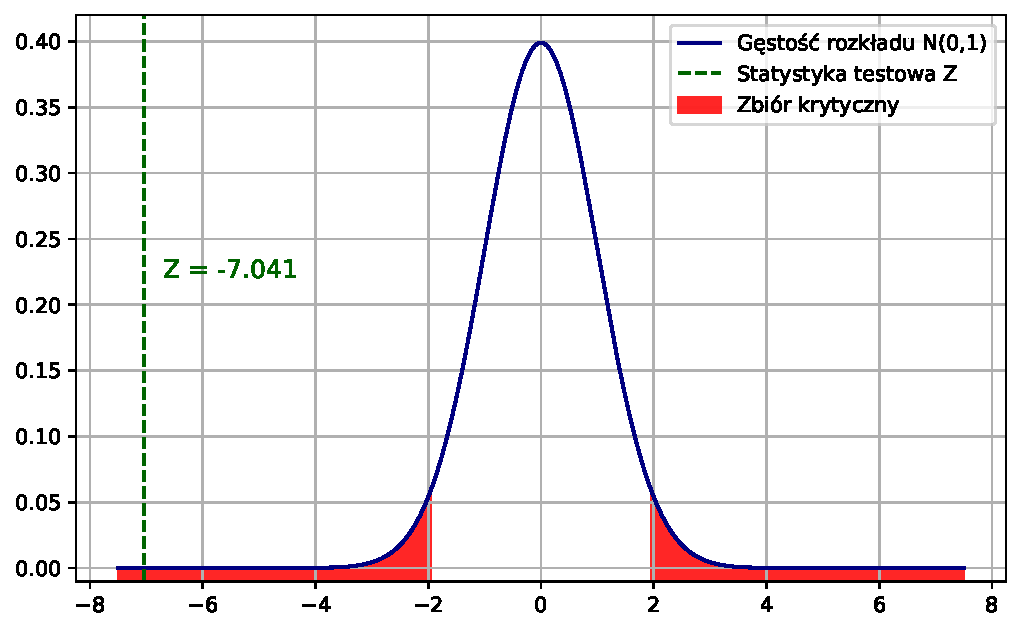
\includegraphics[scale=0.6]{krytyczny1.pdf}
		\caption{Zbiór krytyczny $C$ dla hipotezy zerowej $H_0$, jeśli $H_1 \colon \mu \neq \mu_0$}
	\end{center}
	\end{figure}
	
\noindent P-wartość dla tego podpunktu wynosi $\alpha_p = 2P_{H_0}(Z > |z_{\alpha_p}|) = 2 - 2P_{H_0}(Z \leq |-7.041|) = 2- 2F_Z(7.041) = 1.909 \cdot 10^{-12}$.
	
	
	\subsection{Hipoteza alternatywna $\bm{H_1 \colon \mu > 1.5}$, $\bm{\alpha=0.05}$}
	\noindent Z teorii estymacji przedziałowej dla danych z rozkładu normalnego wiemy, że $P_{H_0}(Z\geq z_{1-\alpha})=\alpha$. Kwantyl rzędu $1-\alpha$ rozkładu $N(0,1)$ wynosi $z_{0.95}=1.6449$. Zbiór krytyczny testu przyjmuje wtedy postać 
	$$C = \left\lbrace Z: Z\geq z_{1-\alpha} \right\rbrace = \left\lbrace Z: Z\geq 1.6449 \right\rbrace .$$ 
	Ponieważ statystyka testowa $Z=-7.041$ jest mniejsza niż $1.6449$, czyli nie znajduje się w przedziale krytycznym, to nie ma podstaw do odrzucenia hipotezy zerowej $H_0$. Zilustrujmy powyższy wniosek.
	
	\begin{figure}[H]
	\begin{center}
		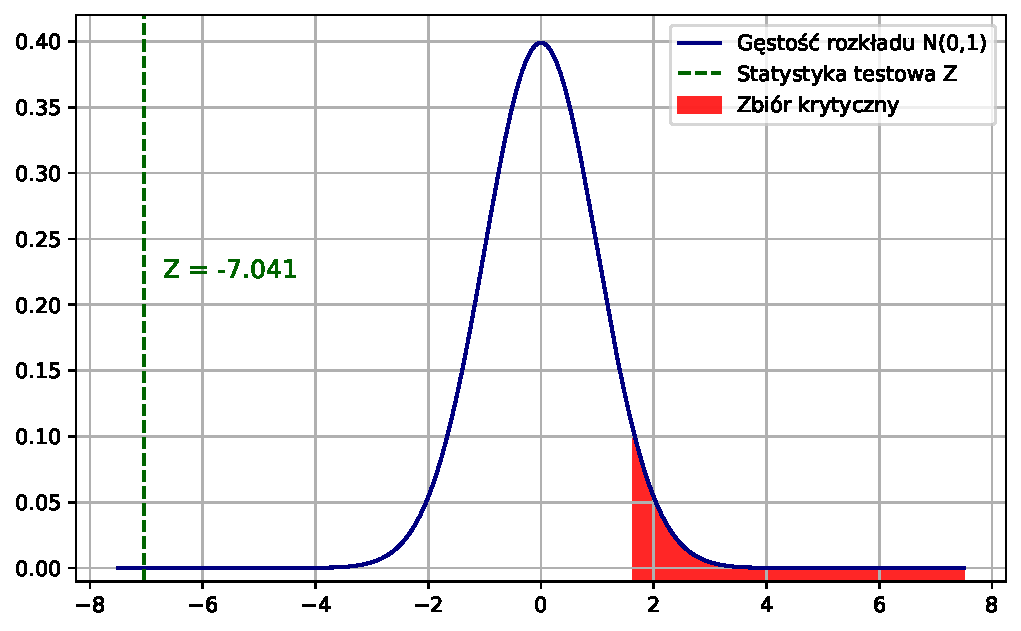
\includegraphics[scale=0.6]{krytyczny2.pdf}
		\caption{Zbiór krytyczny $C$ dla hipotezy zerowej $H_0$, jeśli $H_1 \colon \mu > \mu_0$}
	\end{center}
	\end{figure}
	
\noindent P-wartość dla tego podpunktu wynosi $\alpha_p = P_{H_0}(Z > z_{\alpha_p}) = 1 - P_{H_0}(Z \leq -7.041) = 1 - F_Z(-7.041) \approx 1 $.
	
	
	\subsection{Hipoteza alternatywna $\bm{H_1 \colon \mu < 1.5}$, $\bm{\alpha=0.05}$}
	\noindent Z teorii estymacji przedziałowej dla danych z rozkładu normalnego wiemy, że $P_{H_0}(Z\geq z_{1-\alpha}) = P_{H_0}(Z\leq -z_{1-\alpha})= P_{H_0}(Z\leq z_{\alpha}) = \alpha$. Kwantyl rzędu $\alpha$ rozkładu $N(0,1)$ wynosi $-z_{0.95}=z_{0.05}=-1.6449$. Zbiór krytyczny testu przyjmuje wtedy postać 
	$$C = \left\lbrace Z: Z\leq z_{\alpha} \right\rbrace = \left\lbrace Z: Z\leq -1.6449 \right\rbrace .$$ 
	Ponieważ statystyka testowa $Z=-7.041$ jest mniejsza niż $-1.6449$, czyli wpada do przedziału krytycznego, to odrzucamy hipotezę zerową $H_0$ i przyjmujemy hipotezę alternatywną $H_1$. Zilustrujmy powyższy wniosek.
	
	\begin{figure}[H]
	\begin{center}
		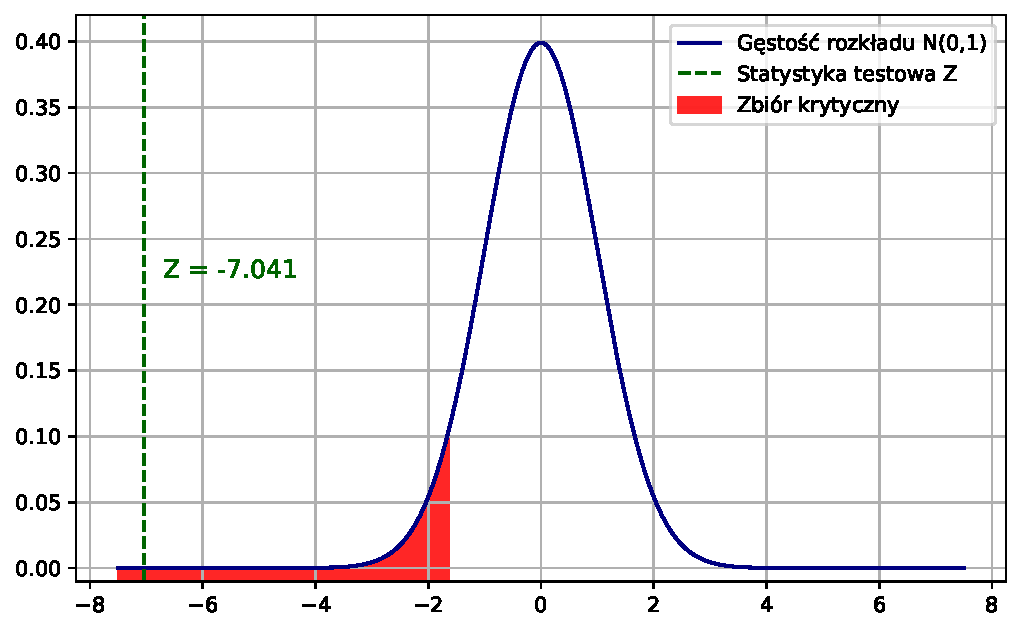
\includegraphics[scale=0.6]{krytyczny3.pdf}
		\caption{Zbiór krytyczny $C$ dla hipotezy zerowej $H_0$, jeśli $H_1 \colon \mu < \mu_0$}
	\end{center}
	\end{figure}
	
\noindent P-wartość dla tego podpunktu wynosi $\alpha_p = P_{H_0}(Z\leq z_{\alpha_p}) = P_{H_0}(Z \leq -7.041) = F_Z(-7.041) = 9.543 \cdot 10^{-13}$. \\

\noindent Przypomnijmy, że poziom istotności $\alpha$ to z definicji miara dokładności wykonywanego testu. Przyjęcie niższego poziomu istotności w powyższych podpunktach spowoduje zmniejszenie przedziału krytycznego, a w konsekwencji zmniejszenie p-wartości. Analogicznie dla zwiększenia poziomu istotności $\alpha$.



	\subsection{Wnioski dla hipotezy $\bm{H_0 \colon \mu = 1.5}$}
	\noindent Podsumujmy zebrane informacje w tabeli:
	
	\begin{table}[H]
    \centering
    \resizebox{\textwidth}{!}{
    \begin{tblr}{|Q[c]|Q[c]|Q[c]|Q[c]|Q[c]|Q[c]|}
    \hline
        Hipoteza $H_1$ & Kwantyle $z$ & Statystyka $Z$ & Zbiór krytyczny $C$ & Hipoteza $H_0$ & P-wartość  \\ \hline
        $\mu \neq 1.5$  & $z_{0.025}=-1.96, z_{0.975}=1.96$ & $-7.041$ & $(-\infty ,-1.96)\cup(1.96,\infty)$ & odrzucona & $1.909 \cdot 10^{-12}$  \\ \hline
        $\mu > 1.5$ & $z_{0.95}=1.6449$ & $-7.041$ & $(1.6449,\infty)$ & przyjęta & $\approx 1 $  \\ \hline
        $\mu < 1.5$ & $z_{0.05}=-1.6449$ & $-7.041$ & $(-\infty,-1.6449)$ & odrzucona & $9.543 \cdot 10^{-13}$  \\ \hline
    \end{tblr}
    }
\end{table}

\noindent Biorąc pod uwagę przyjmowane hipotezy alternatywne $H_1$, możemy wysnuć wniosek, że nasze dane pochodzą z rozkładu normalnego, gdzie $\mu$ ma wartość mniejszą niż $1.5$. Zgadza się to z p-wartością bliską $1$ przy $H_1 \colon \mu >1.5$.
	
	
	
	\section{Zadanie 2}
	\subsection{Wstęp}
\noindent Hipotezą zerową nazywamy założenie, że wariancja $\sigma^{2}$ naszych danych wyniesie $1.5$. Hipotezę tę oznaczamy symbolem $H_0$ i piszemy $H_0 \colon \sigma^{2} = \sigma_0^2 = 1.5$. Drugą hipotezę nazywamy hipotezą alternatywną i oznaczamy ją przez $H_1$. W naszym przypadku:
	\begin{enumerate}[label=(\alph*)]
		\item $H_1 \colon \sigma^{2} \neq \sigma^{2}_0$
		\item $H_1 \colon \sigma^{2} > \sigma^{2}_0$
		\item $H_1 \colon \sigma^{2} < \sigma^{2}_0$. \\
	\end{enumerate} 
	
	
\noindent Jeśli zachodzi hipoteza zerowa, to nasze dane mają rozkład $N(0.2,\sqrt{1.5})$. Zauważmy, że parametr $\mu$ jest znany i wynosi $0.2$. Do weryfikacji $H_0$ będziemy potrzebować jakiejś statystyki testowej. W celu zbadania wariancji w rodzinie rozkładów normalnych używa się statystyki 
$$\chi^2 = \frac{(n-1)S^2}{\sigma_0^2}, \qquad \mathrm{gdzie} \hspace{2mm} S^2 = \frac{1}{n-1} \sum_{i=1}^{n}(\mu-x_i)^2.$$  
	
	\noindent Ta zmienna losowa $\chi^2$ ma rozkład $\chi^2$ z $(n-1)$ stopniami swobody. Gdy hipoteza zerowa $H_0$ jest fałszywa, wzór na statystykę $\chi^2$ można zapisać następująco:
$$\chi^2 = \frac{(n-1)S^2}{\sigma_0^2} = \underbrace{\frac{(n-1)S^2}{\sigma^2}}_{\sim \chi^2_{n-1}} \cdot \frac{\sigma^2}{\sigma_0^2}.$$

	\noindent Ze wzoru widać, że kluczem do weryfikacji hipotezy jest sprawdzenie czy statystyka $\chi^2$ przyjmuje wartości charakterystyczne dla jej założonego rozkładu $\chi^2_{n-1}$. Jeśli nie, to niepoprawny będzie również rozkład $N(0.2,\sqrt{1.5})$ przewidywany dla naszych danych, a tym samym odrzucimy hipotezę zerową. Zbiór liczb, które prowadzą do odrzucenia hipotezy $H_0$ na korzyść $H_1$ nazywamy zbiorem krytycznym $C$. Jego rozmiar zależy od miary dokładności wykonywanego testu, czyli tzw. poziomu istotności. Wyznacza on prawdopodobieństwo popełnienia błędu pierwszego rodzaju - odrzucenia hipotezy zerowej, gdy jest ona prawdziwa. Poziom istotności oznaczamy poprzez symbol $\alpha$. W zadaniu przyjmujemy, że jest on równy $0.05$. \\
	
	
	\noindent Wprowadźmy jeszcze pojęcie p-wartości. Jest to najmniejszy poziom istotności $\alpha$, przy którym zaobserwowana wartość statystyki testowej $\chi^2$ prowadzi do odrzucenia hipotezy zerowej $H_0$.



	\subsection{Hipoteza alternatywna $\bm{H_1 \colon \sigma^2 \neq 1.5}$, $\bm{\alpha=0.05}$}
	\noindent Z teorii estymacji przedziałowej dla danych z rozkładu normalnego wiemy, że $P_{H_0}(x_{\frac{\alpha}{2}} \leq \chi^2 \leq x_{1-\frac{\alpha}{2}})=1 - \alpha$. Powyższe kwantyle rozkładu $\chi^2_{n-1}$ wynoszą $x_{0.025}=913.3$ oraz $x_{0.975}=1088.49$. Zbiór krytyczny testu przyjmuje wtedy postać
$$C = \left\lbrace \chi^2: \chi^2\leq x_{\frac{\alpha}{2}} \vee \chi^2\geq x_{1-\frac{\alpha}{2}} \right\rbrace = \left\lbrace \chi^2: \chi^2\leq 913.3 \vee \chi^2\geq 1088.49 \right\rbrace.$$ 

\noindent Ponieważ statystyka testowa $\chi^2$ wynosi $1110.968$, czyli znajduje się w przedziale krytycznym, to odrzucamy hipotezę zerową $H_0$ i przyjmujemy hipotezę alternatywną $H_1$. Zilustrujmy powyższy wniosek.

	\begin{figure}[H]
	\begin{center}
		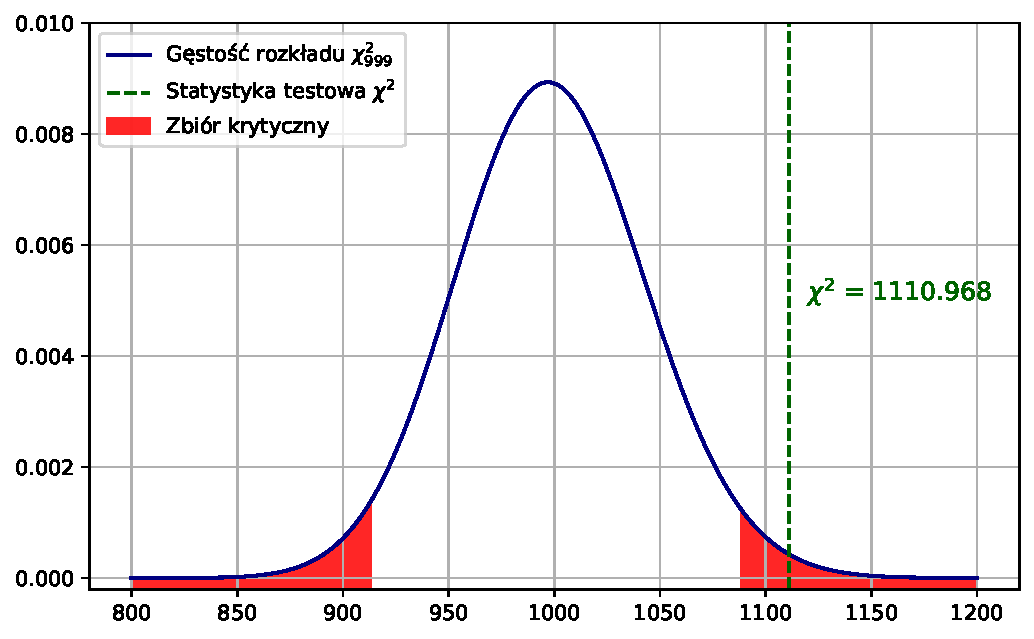
\includegraphics[scale=0.6]{krytyczny4.pdf}
		\caption{Zbiór krytyczny $C$ dla hipotezy zerowej $H_0$, jeśli $H_1 \colon \sigma^2 \neq 1.5$}
	\end{center}
	\end{figure}


\noindent P-wartość dla tego podpunktu wynosi $\alpha_p = 2P_{H_0}(\chi^2 > |x_{\alpha_p}|) = 2 - 2P_{H_0}(\chi^2 \leq |x_{\alpha_p}|) = 2- 2F_{\chi^2_{999}}(1110.968) = 0.015$.



	\subsection{Hipoteza alternatywna $\bm{H_1 \colon \sigma^2 > 1.5}$, $\bm{\alpha=0.05}$}
	\noindent Z teorii estymacji przedziałowej dla danych z rozkładu normalnego wiemy, że $P_{H_0}(\chi^2 \geq x_{1-\alpha})=\alpha$. Kwantyl rzędu $1-\alpha$ rozkładu $\chi^2_{999}$ wynosi $x_{0.95}=1073.64$. Zbiór krytyczny testu przyjmuje wtedy postać 
	$$C = \left\lbrace \chi^2: \chi^2\geq x_{1-\alpha} \right\rbrace = \left\lbrace \chi^2: \chi^2 \geq 1073.64 \right\rbrace .$$ 
	
\noindent Ponieważ statystyka testowa $\chi^2=1110.968$ jest większa niż $1073.64$, czyli wpada do przedziału krytycznego, to odrzucamy hipotezę zerową $H_0$ i przyjmujemy hipotezę alternatywną $H_1$. Zilustrujmy powyższy wniosek.

	\begin{figure}[H]
	\begin{center}
		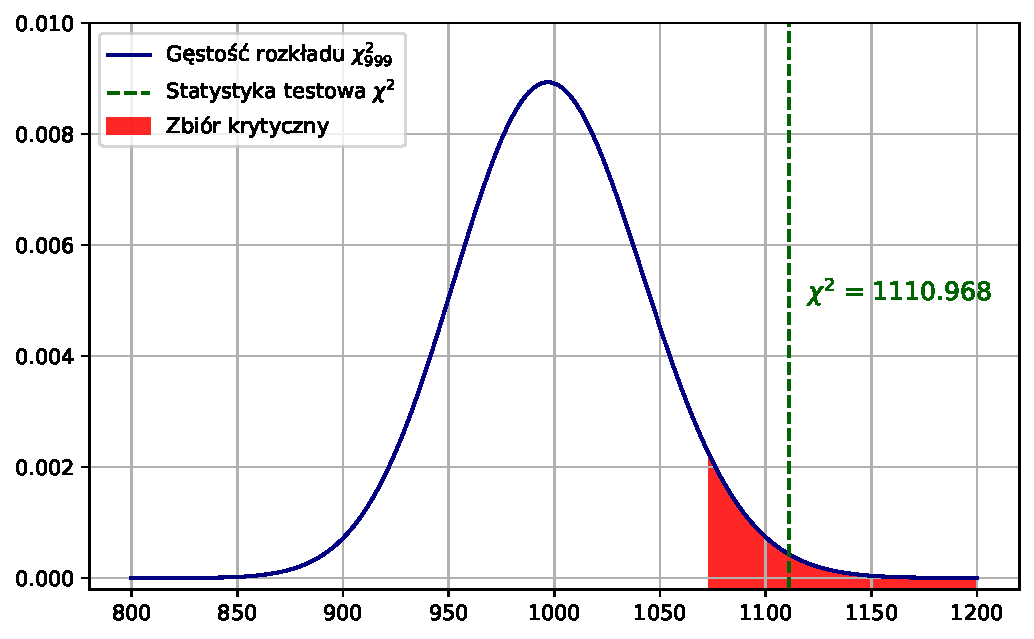
\includegraphics[scale=0.6]{krytyczny5.pdf}
		\caption{Zbiór krytyczny $C$ dla hipotezy zerowej $H_0$, jeśli $H_1 \colon \sigma^2 > 1.5$}
	\end{center}
	\end{figure}

\noindent P-wartość dla tego podpunktu wynosi $\alpha_p = P_{H_0}(\chi^2 > x_{\alpha_p}) = 1 - P_{H_0}(\chi^2 \leq 1110.968) = 1 - F_{\chi^2_{999}}(1110.968) = 0.0075$.



	\subsection{Hipoteza alternatywna $\bm{H_1 \colon \sigma^2 < 1.5}$, $\bm{\alpha=0.05}$}
	\noindent Z teorii estymacji przedziałowej dla danych z rozkładu normalnego wiemy, że $P_{H_0}(\chi^2 \geq x_{1-\alpha})=P_{H_0}(\chi^2 \leq x_{\alpha})=\alpha$. Kwantyl rzędu $\alpha$ rozkładu $\chi^2_{999}$ wynosi $x_{0.05}=926.63$. Zbiór krytyczny testu przyjmuje wtedy postać 
	$$C = \left\lbrace \chi^2: \chi^2 \leq x_{\alpha} \right\rbrace = \left\lbrace \chi^2: \chi^2 \leq 926.63 \right\rbrace .$$ 
	
\noindent Ponieważ statystyka testowa $\chi^2=1110.968$ jest większa niż $926.63$, czyli nie znajduje się w przedziale krytycznym, to nie ma podstaw do odrzucenia hipotezy zerowej $H_0$. Zilustrujmy powyższy wniosek.

	\begin{figure}[H]
	\begin{center}
		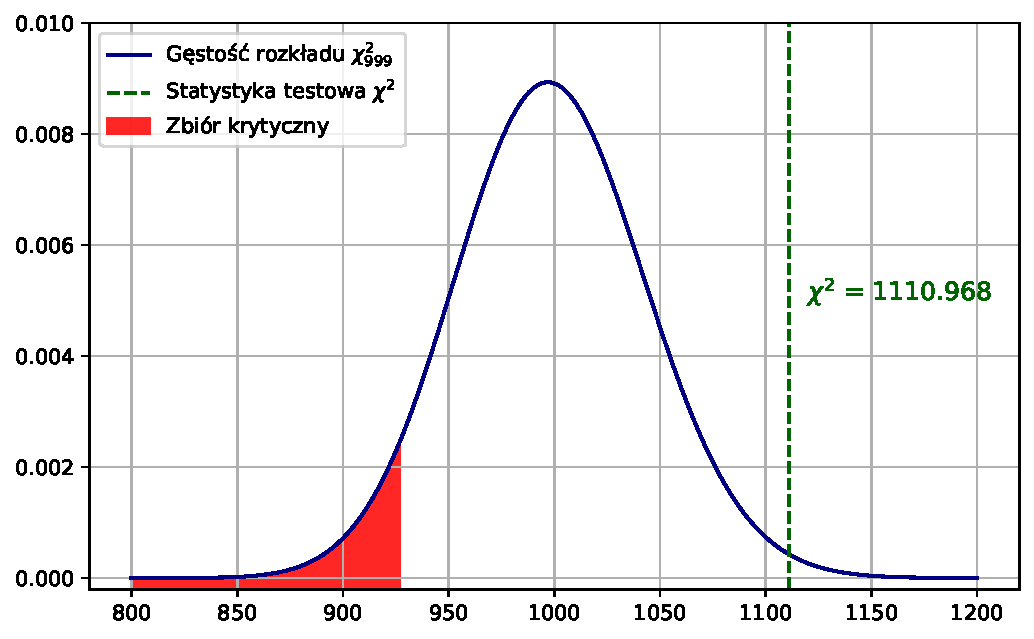
\includegraphics[scale=0.6]{krytyczny6.pdf}
		\caption{Zbiór krytyczny $C$ dla hipotezy zerowej $H_0$, jeśli $H_1 \colon \sigma^2 < 1.5$}
	\end{center}
	\end{figure}

\noindent P-wartość dla tego podpunktu wynosi $\alpha_p = P_{H_0}(\chi^2 \leq x_{\alpha_p}) = P_{H_0}(\chi^2 \leq 1110.968) = F_{\chi^2} (1110.968) = 0.992$. \\

\noindent Przypomnijmy, że poziom istotności $\alpha$ to z definicji miara dokładności wykonywanego testu. Przyjęcie niższego poziomu istotności w powyższych podpunktach spowoduje zmniejszenie przedziału krytycznego, a w konsekwencji zmniejszenie p-wartości. Analogicznie dla zwiększenia poziomu istotności $\alpha$.


	\subsection{Wnioski dla hipotezy $\bm{H_0 \colon \sigma^2 = 1.5}$}
	\noindent Podsumujmy zebrane informacje w tabeli:
	
	\begin{table}[H]
    \centering
    \resizebox{\textwidth}{!}{
    \begin{tblr}{|Q[c]|Q[c]|Q[c]|Q[c]|Q[c]|Q[c]|}
    \hline
        Hipoteza $H_1$ & Kwantyle $x$ & Statystyka $\chi^2$ & Zbiór krytyczny $C$ & Hipoteza $H_0$ & P-wartość  \\ \hline
        $\sigma^2 \neq 1.5$  & $x_{0.025}=913.3, x_{0.975}=1088.49$ & $1110.968$ & $(-\infty ,913.3)\cup(1088.49,\infty)$ & odrzucona & $0.015$  \\ \hline
        $\sigma^2 > 1.5$ & $x_{0.95}=1073.64$ & $1110.968$ & $(1073.64,\infty)$ & odrzucona & $0.0075$  \\ \hline
        $\sigma^2 < 1.5$ & $x_{0.05}=926.63$ & $1110.968$ & $(-\infty,926.63)$ & przyjęta & $0.992$  \\ \hline
    \end{tblr}
    }
\end{table}

\noindent Biorąc pod uwagę przyjmowane hipotezy alternatywne $H_1$, możemy wysnuć wniosek, że nasze dane pochodzą z rozkładu normalnego, gdzie $\sigma^2$ ma wartość większą niż $1.5$. Zgadza się to z p-wartością bliską $1$ przy $H_1 \colon \sigma^2 <1.5$.



	\section{Zadanie 3}
	\subsection{Wstęp}
	\noindent Błąd pierwszego rodzaju to prawdopodobieństwo odrzucenia hipotezy zerowej, gdy ta jest prawdziwa. Jego teoretyczna wartość jest równa poziomowi istotności $\alpha$. Aby wyznaczyć symulacyjnie błąd I rodzaju musimy wygenerować prostą próbę losową z rozkładu normalnego o parametrach zgodnych z $H_0$ ($\mu = 1.5$ oraz $\sigma = 0.2$) i sprawdzić ile razy odrzucimy hipotezę zerową. Algorytm:
	
	\begin{enumerate}
		\itemsep 3mm
		\item Ustalamy $\alpha = 0.05, n = 1000$
		\item Generujemy $X_1, \dotsc, X_n$ - prostą próbę losową z rozkładu $N(\mu,\sigma)$ (parametry zgodne z $H_0$)
		\item Wyznaczamy wartość statystyki testowej $Z$ lub $\chi^2$
		\item Wyznaczamy obszar krytyczny (jego postać zależy od hipotezy alternatywnej $H_1$)
		\item Sprawdzamy, czy statystyka $Z$ lub $\chi^2$ jest w obszarze krytycznym
		\item Powtarzamy kroki od $2)$ do $5)$ N = 1000 razy i zliczamy ile razy statystyka $Z$ lub $\chi^2$ jest w obszarze krytycznym
		\item Ilość $Z$ (lub $\chi^2$) w obszarze krytycznym podzielone przez $N$ to w przybliżeniu błąd I rodzaju \\
	\end{enumerate}

	\noindent Błąd drugiego rodzaju to prawdopodobieństwo przyjęcia fałszywej hipotezy zerowej i odrzucenia prawdziwej hipotezy alternatywnej. Jego wartość zależy m.in. od tego jak daleko jesteśmy od hipotezy zerowej, tzn. ile wynosi wartość parametru $\mu$ (lub $\sigma^2$). Aby wyznaczyć symulacyjnie błąd II rodzaju musimy wygenerować prostą próbę losową z rozkładu normalnego o parametrach zgodnych z $H_1$ (ale blisko tych z $H_0$) i sprawdzić ile razy przyjmujemy hipotezę zerową. Algorytm:
	
	\begin{enumerate}
		\itemsep 3mm
		\item Ustalamy $\alpha = 0.05, n = 1000$. Wartości parametrów $\mu$ i $\sigma$ dobieramy zgodnie z hipotezą alternatywną $H_1$, ale blisko hipotezy zerowej $H_0$ - przykładowo oddalone maksymalnie o 0.03 od wartości z $H_0$)
		\item Generujemy $X_1, \dotsc, X_n$ - prostą próbę losową z rozkładu $N(\mu,\sigma)$
		\item Wyznaczamy wartość statystyki testowej $Z$ lub $\chi^2$
		\item Wyznaczamy obszar krytyczny (jego postać zależy od hipotezy alternatywnej $H_1$)
		\item Sprawdzamy, czy statystyka $Z$ lub $\chi^2$ jest poza obszarem krytycznym
		\item Powtarzamy kroki od $2)$ do $5)$ N = 1000 razy i zliczamy ile razy statystyka $Z$ lub $\chi^2$ jest poza obszarem krytycznym
		\item Ilość $Z$ (lub $\chi^2$) poza obszarem krytycznym podzielone przez $N$ to w przybliżeniu błąd II rodzaju \\
	\end{enumerate}
	
	
	\subsection{Wyniki symulacji błędu I rodzaju dla testów $\bm{\mu$}}
	
	\begin{figure}[H]
	\begin{center}
		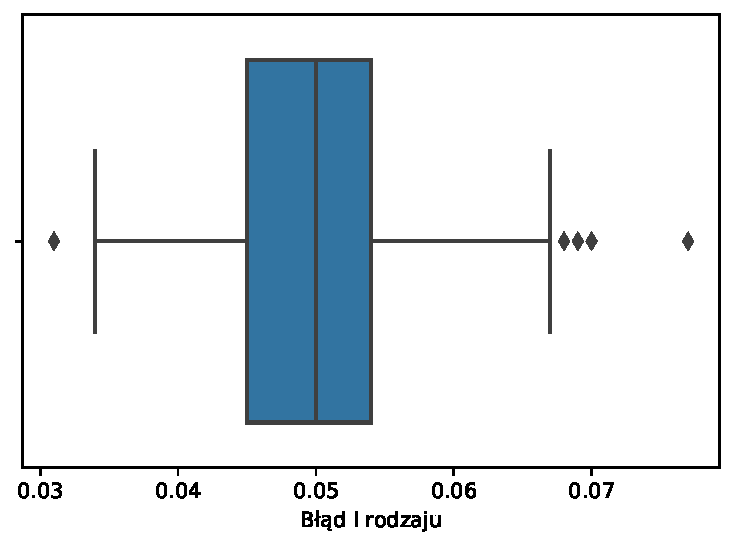
\includegraphics[scale=0.6]{box1.pdf}
		\caption{Wykres pudełkowy przedstawiający wartości błędów I rodzaju dla $\mu$ przy hipotezie alternatywnej $H_1 \colon \mu \neq 1.5$}
	\end{center}
	\end{figure}
	
	
	\begin{figure}[H]
	\begin{center}
		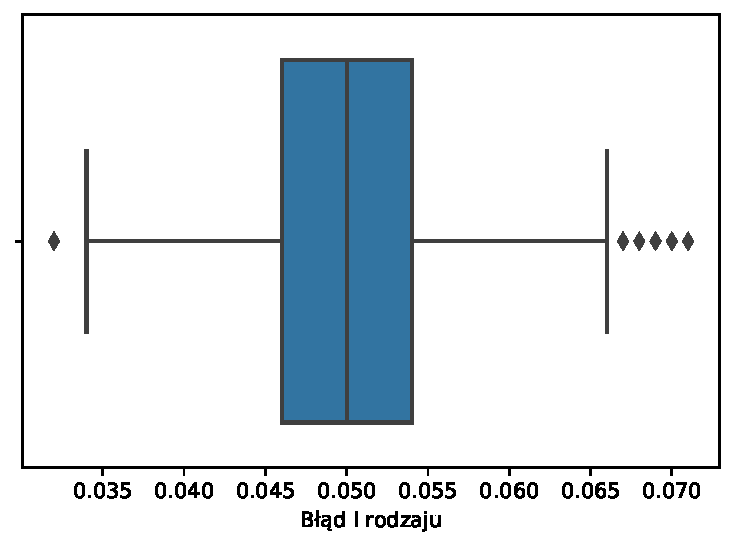
\includegraphics[scale=0.6]{box2.pdf}
		\caption{Wykres pudełkowy przedstawiający wartości błędów I rodzaju dla $\mu$ przy hipotezie alternatywnej $H_1 \colon \mu > 1.5$}
	\end{center}
	\end{figure}
	
	
	\begin{figure}[H]
	\begin{center}
		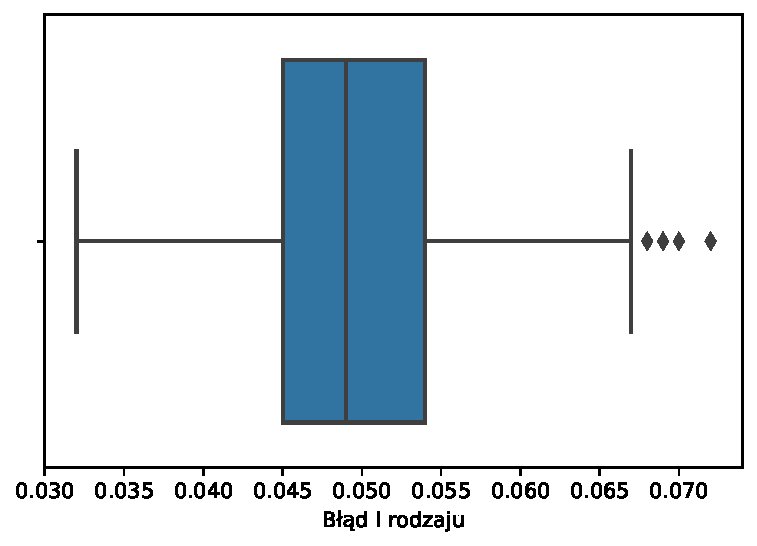
\includegraphics[scale=0.6]{box3.pdf}
		\caption{Wykres pudełkowy przedstawiający wartości błędów I rodzaju dla $\mu$ przy hipotezie alternatywnej $H_1 \colon \mu < 1.5$}
	\end{center}
	\end{figure}


	
	\subsection{Wyniki symulacji błędu I rodzaju dla testów $\bm{\sigma^2}$}
	
	\begin{figure}[H]
	\begin{center}
		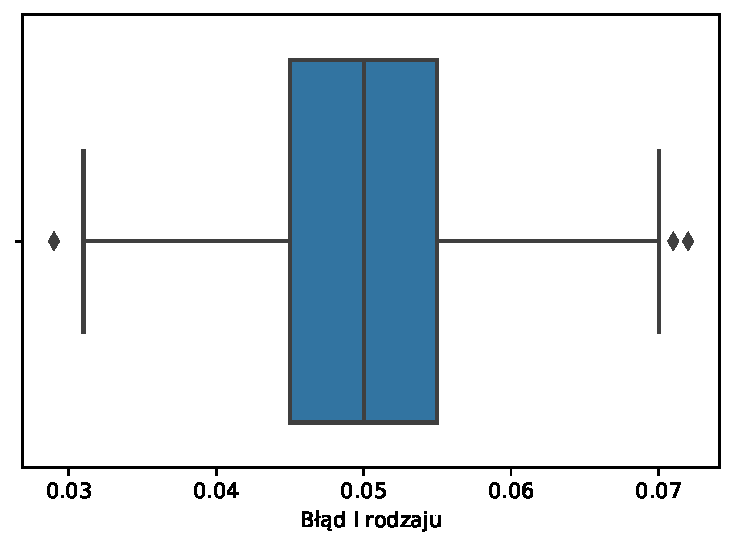
\includegraphics[scale=0.6]{box4.pdf}
		\caption{Wykres pudełkowy przedstawiający wartości błędów I rodzaju dla $\sigma^2$ przy hipotezie alternatywnej $H_1 \colon \sigma^2 \neq 1.5$}
	\end{center}
	\end{figure}
	
	
	\begin{figure}[H]
	\begin{center}
		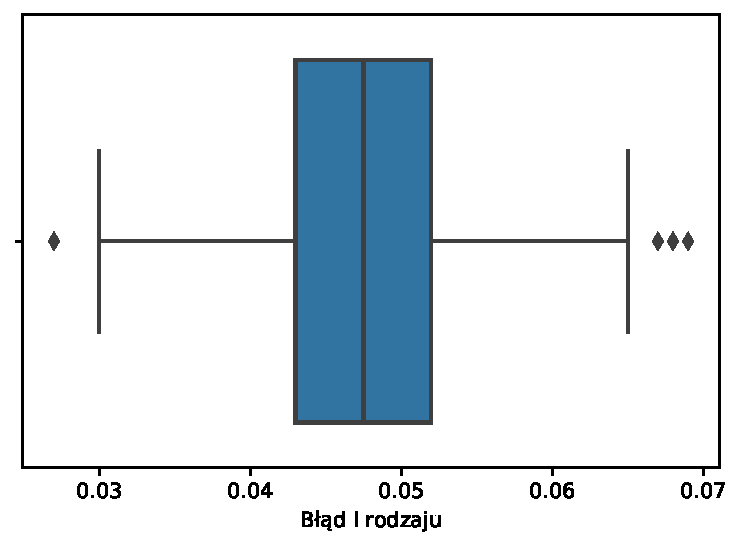
\includegraphics[scale=0.6]{box5.pdf}
		\caption{Wykres pudełkowy przedstawiający wartości błędów I rodzaju dla $\sigma^2$ przy hipotezie alternatywnej $H_1 \colon \sigma^2 > 1.5$}
	\end{center}
	\end{figure}
	
	
	\begin{figure}[H]
	\begin{center}
		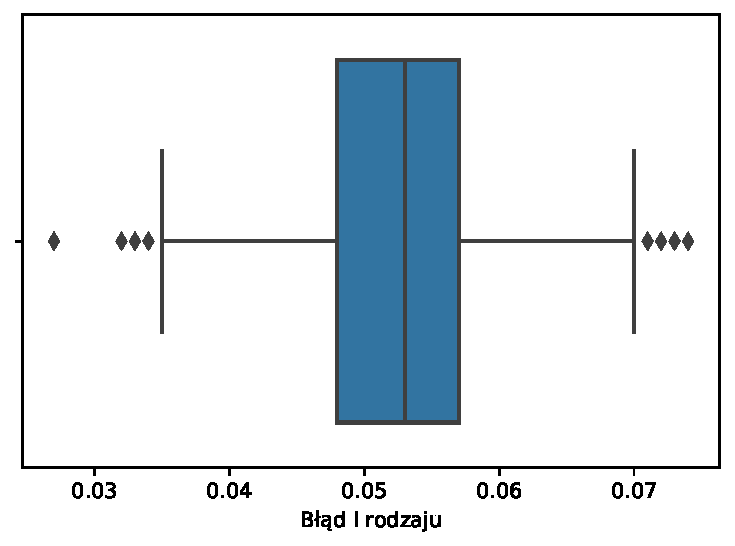
\includegraphics[scale=0.6]{box6.pdf}
		\caption{Wykres pudełkowy przedstawiający wartości błędów I rodzaju dla $\sigma^2$ przy hipotezie alternatywnej $H_1 \colon \sigma^2 < 1.5$}
	\end{center}
	\end{figure}
	
	
	\subsection{Wnioski dla symulacji błędów I rodzaju}
	\noindent Wartości wszystkich wykresów pudełkowych oscylują wokół $0.05$. Tyle samo wynosi poziom istotności $\alpha$, czyli teoretyczna wartość błędu I rodzaju. Możemy zatem wnioskować, że testy zostały przeprowadzone poprawnie.
	
	
	
	\subsection{Wyniki symulacji błędu II rodzaju dla testów $\bm{\mu}$}
	
	\begin{figure}[H]
	\begin{center}
		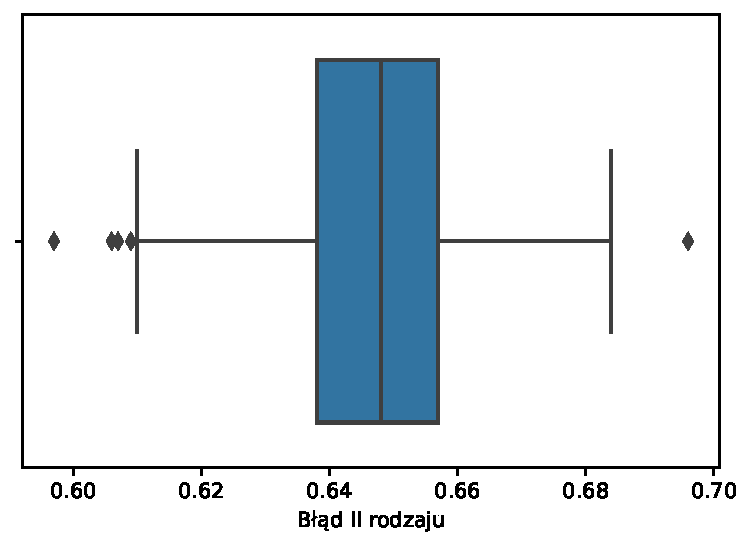
\includegraphics[scale=0.6]{box7.pdf}
		\caption{Wykres pudełkowy przedstawiający wartości błędów II rodzaju dla $\mu=1.51$ przy hipotezie alternatywnej $H_1 \colon \mu \neq 1.5$}
	\end{center}
	\end{figure}
	
	
	\begin{figure}[H]
	\begin{center}
		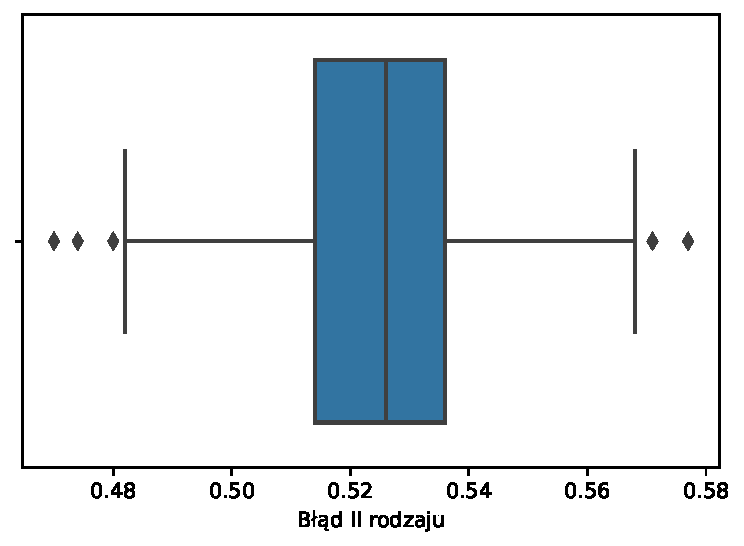
\includegraphics[scale=0.6]{box8.pdf}
		\caption{Wykres pudełkowy przedstawiający wartości błędów II rodzaju dla $\mu=1.51$ przy hipotezie alternatywnej $H_1 \colon \mu > 1.5$}
	\end{center}
	\end{figure}
	
	\begin{figure}[H]
	\begin{center}
		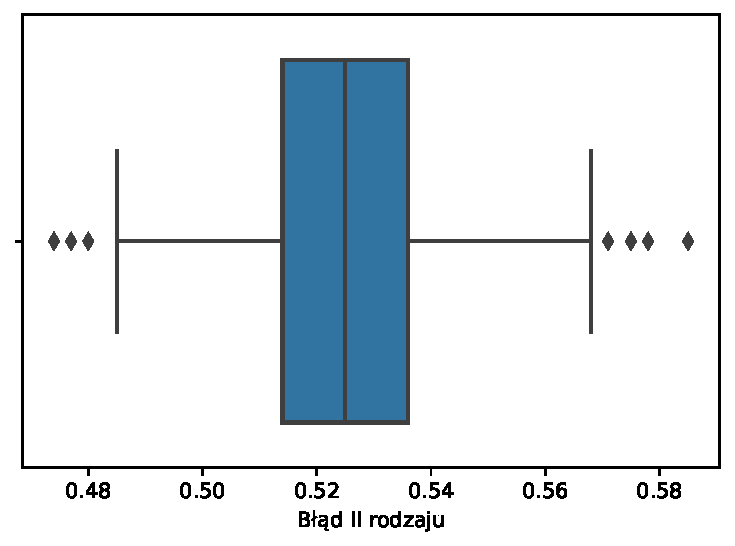
\includegraphics[scale=0.6]{box9.pdf}
		\caption{Wykres pudełkowy przedstawiający wartości błędów II rodzaju dla testów $\mu=1.49$ przy hipotezie alternatywnej $H_1 \colon \mu < 1.5$}
	\end{center}
	\end{figure}
	
	
	
	\subsection{Wyniki symulacji błędu II rodzaju dla testów $\bm{\sigma^2}$}
	
	\begin{figure}[H]
	\begin{center}
		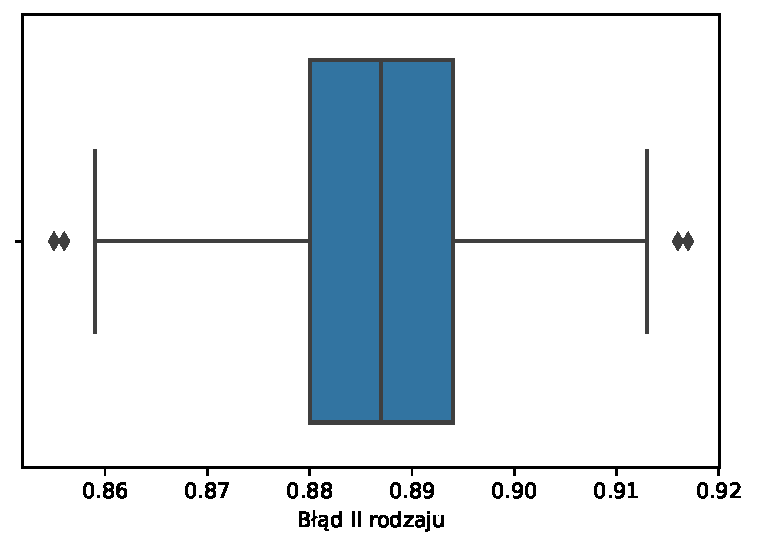
\includegraphics[scale=0.6]{box10.pdf}
		\caption{Wykres pudełkowy przedstawiający wartości błędów II rodzaju dla $\sigma^2=1.55$ przy hipotezie alternatywnej $H_1 \colon \sigma^2 \neq 1.5$}
	\end{center}
	\end{figure}
	
	\begin{figure}[H]
	\begin{center}
		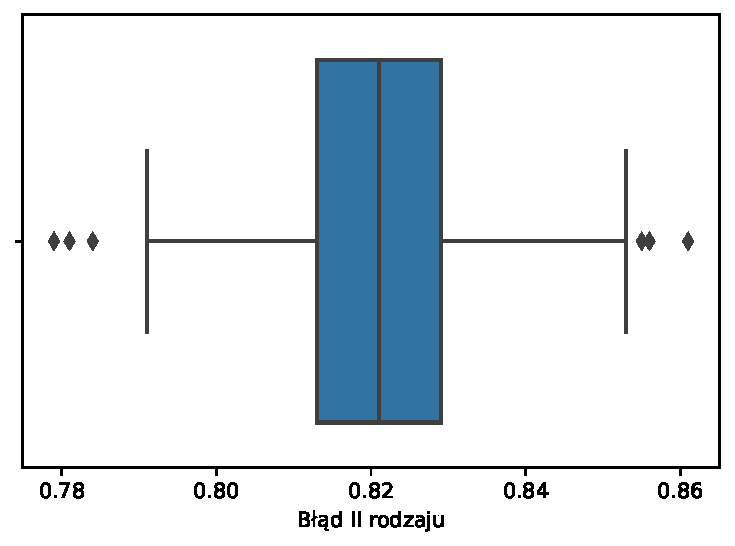
\includegraphics[scale=0.6]{box11.pdf}
		\caption{Wykres pudełkowy przedstawiający wartości błędów II rodzaju dla $\sigma^2=1.55$ przy hipotezie alternatywnej $H_1 \colon \sigma^2 > 1.5$}
	\end{center}
	\end{figure}
	
	\begin{figure}[H]
	\begin{center}
		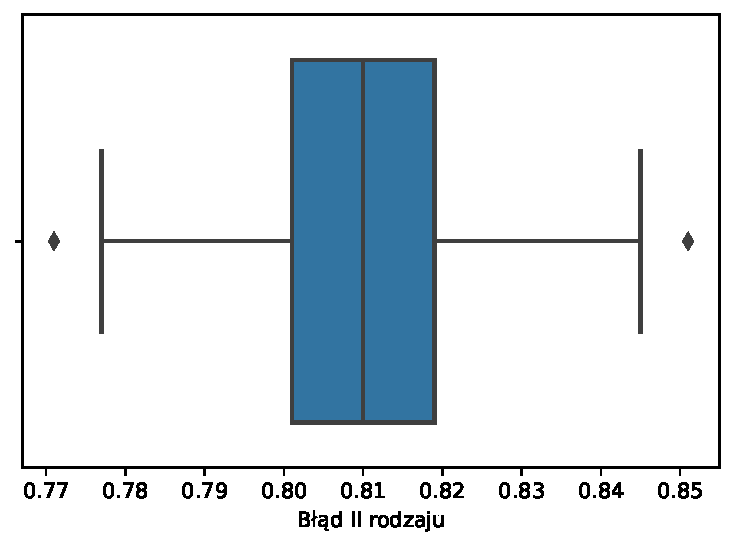
\includegraphics[scale=0.6]{box12.pdf}
		\caption{Wykres pudełkowy przedstawiający wartości błędów II rodzaju dla $\sigma^2 = 1.45$ przy hipotezie alternatywnej $H_1 \colon \sigma^2 < 1.5$}
	\end{center}
	\end{figure}
	
	
	\subsection{Wnioski dla symulacji błędów II rodzaju}
	\noindent Podsumujmy zebrane informacje w tabelach.
	
	\begin{table}[H]
    \centering
    \resizebox{\textwidth}{!}{
    \begin{tblr}{|Q[c]|Q[c]|Q[c]|Q[c]|}
    \hline
        Hipoteza alternatywna $H_1$ & $\mu$ & Wartość średnia błędu II rodzaju & Średnia moc testu  \\ \hline
        $\mu \neq 1.5$  & $1.51$ & 0.64722 & 0.35278  \\ \hline
        $\mu > 1.5$ & $1.51$ & 0.525405 & 0.474595  \\ \hline
        $\mu < 1.5$ & $1.49$ & 0.525083 & 0.474917  \\ \hline
    \end{tblr}
    }
	\end{table}
	
	\begin{table}[H]
    \centering
    \resizebox{\textwidth}{!}{
    \begin{tblr}{|Q[c]|Q[c]|Q[c]|Q[c]|}
    \hline
        Hipoteza alternatywna $H_1$ & $\sigma^2$ & Wartość średnia błędu II rodzaju & Średnia moc testu  \\ \hline
        $\sigma^2 \neq 1.5$  & $1.55$ & $0.886972$ & $0.113028$  \\ \hline
        $\sigma^2 > 1.5$ & $1.55$ & 0.82109 & 0.17891  \\ \hline
        $\sigma^2 < 1.5$ & $1.45$ & 0.809961 & 0.190039  \\ \hline
    \end{tblr}
    }
	\end{table}
	
	\noindent Zauważmy, że wartość średnia błędu II rodzaju i średnia moc testu sumują się do 1. Dwa ostatnie rzędy pierwszej tabeli przyjmują podobne wartości ze względu na dobór parametrów i symetrię rozkładu normalnego.
	
\end{document}
